\documentclass[10pt,twocolumn]{article}
\usepackage[margin=1.8 cm]{geometry}
\setlength{\columnsep}{0.7 cm}

\usepackage[]{graphicx}
\usepackage[skip=10pt,font=scriptsize]{caption,subcaption}

\usepackage[usenames, dvipsnames]{color}

\usepackage{amsmath}
\usepackage{amssymb}

\graphicspath{{bbfigs/}}

\begin{document}

\subsection*{Cryogenic temperatures}

- \textcolor{RoyalPurple}{Purple:} statements/words that don't seem so necessary or that should be clearly modified/expanded.

\noindent
- \textcolor{ForestGreen}{Green:} my comments.

\vspace{0.25cm}

As pointed out in the previous \textcolor{RoyalPurple}{(sub-)}section, \textcolor{RoyalPurple}{for a sufficiently large atom density}\footnote{\textcolor{ForestGreen}{\ldots because 1/$b_{nL}N_b$ might not be the right scaling when the atom density is small. The right scaling could be, for example, $1/\sqrt{1+(b_{nL}N_b)^2}$.}} the time until the creation of the first contaminant atom is \textcolor{RoyalPurple}{[301]}

\begin{displaymath}
\tau_c = \frac{4\delta^2}{\Omega^2}\frac{\tau_0}{b_{nL}N_{\beta}} \textcolor{RoyalPurple}{\text{\; (or} \sim \text{ instead of } = \text{)}},
\end{displaymath}

\noindent
where $N_{\beta}$ is the number of atoms per effective interaction volume $\beta$, and $b_{nL}$ is the sum of the branching ratios from the $nL$ Rydberg state to the \textcolor{RoyalPurple}{relevant\footnote{\textcolor{ForestGreen}{We've made the slightly arbitrary choice that the relevant ones are those that contribute the most to the value of $\beta$.}}} contaminant states. \textcolor{RoyalPurple}{$\tau_0$ is the natural lifetime of the  $nL$  state. If $\beta$ is much larger than the size of the sample, $N_{\beta}$ is simply the total number of atoms $N_0$.}

The time $\tau_c$ depends on the ambient temperature\footnote{\textcolor{ForestGreen}{this is the temperature defining the spectrum of black-body radiation surrounding the sample.}} $T$ through $\tau_0$ and $b_{nL}$. Using the estimates from [302] and the quasiclassical formulas in [303], we  \textcolor{RoyalPurple}{\textit{roughly}}\footnote{\textcolor{ForestGreen}{I think it should be ``roughly'' if $\tau_c \sim$ and not $\tau_c =$.}} estimate the largest value $T_N^*$ of the ambient temperature $T$ needed to \textcolor{RoyalPurple}{compensate} for the avalanche dephasing effect as a function of $N_{\beta}$.


In figure \ref{fig:cthcal_4} we plot $\tau_0$, $b_{nL}$ and $T_N^*$ as a function of $T$ for different $^{87}$Rb $nS$ Rydberg states.

Rydberg-dressing proposals \textcolor{RoyalPurple}{like} [304,305] and previous experimental setups [306] making use of systems with an \textcolor{ForestGreen}{\textit{effective}} $N_{\beta}\lesssim$ 40 would need an ambient temperature between 10 K and 30 K to make up for the dephasing effect. The effects on those with a low atom number $N\sim 10$ [309] should be negligible for cryogenic temperatures around 70 K.

\textcolor{RoyalPurple}{Proposals like [307] and [308] where the atom number is 100-1000 atoms but the van der Waals blockade radius is larger than or comparable to the sample dimensions will not be considerably affected by this dephasing process (even if not working in a cryogenic environment).}

\begin{figure}[]
\begin{minipage}[c][6.4cm][t]{.14\textwidth}
  \vspace*{\fill}
  \centering
  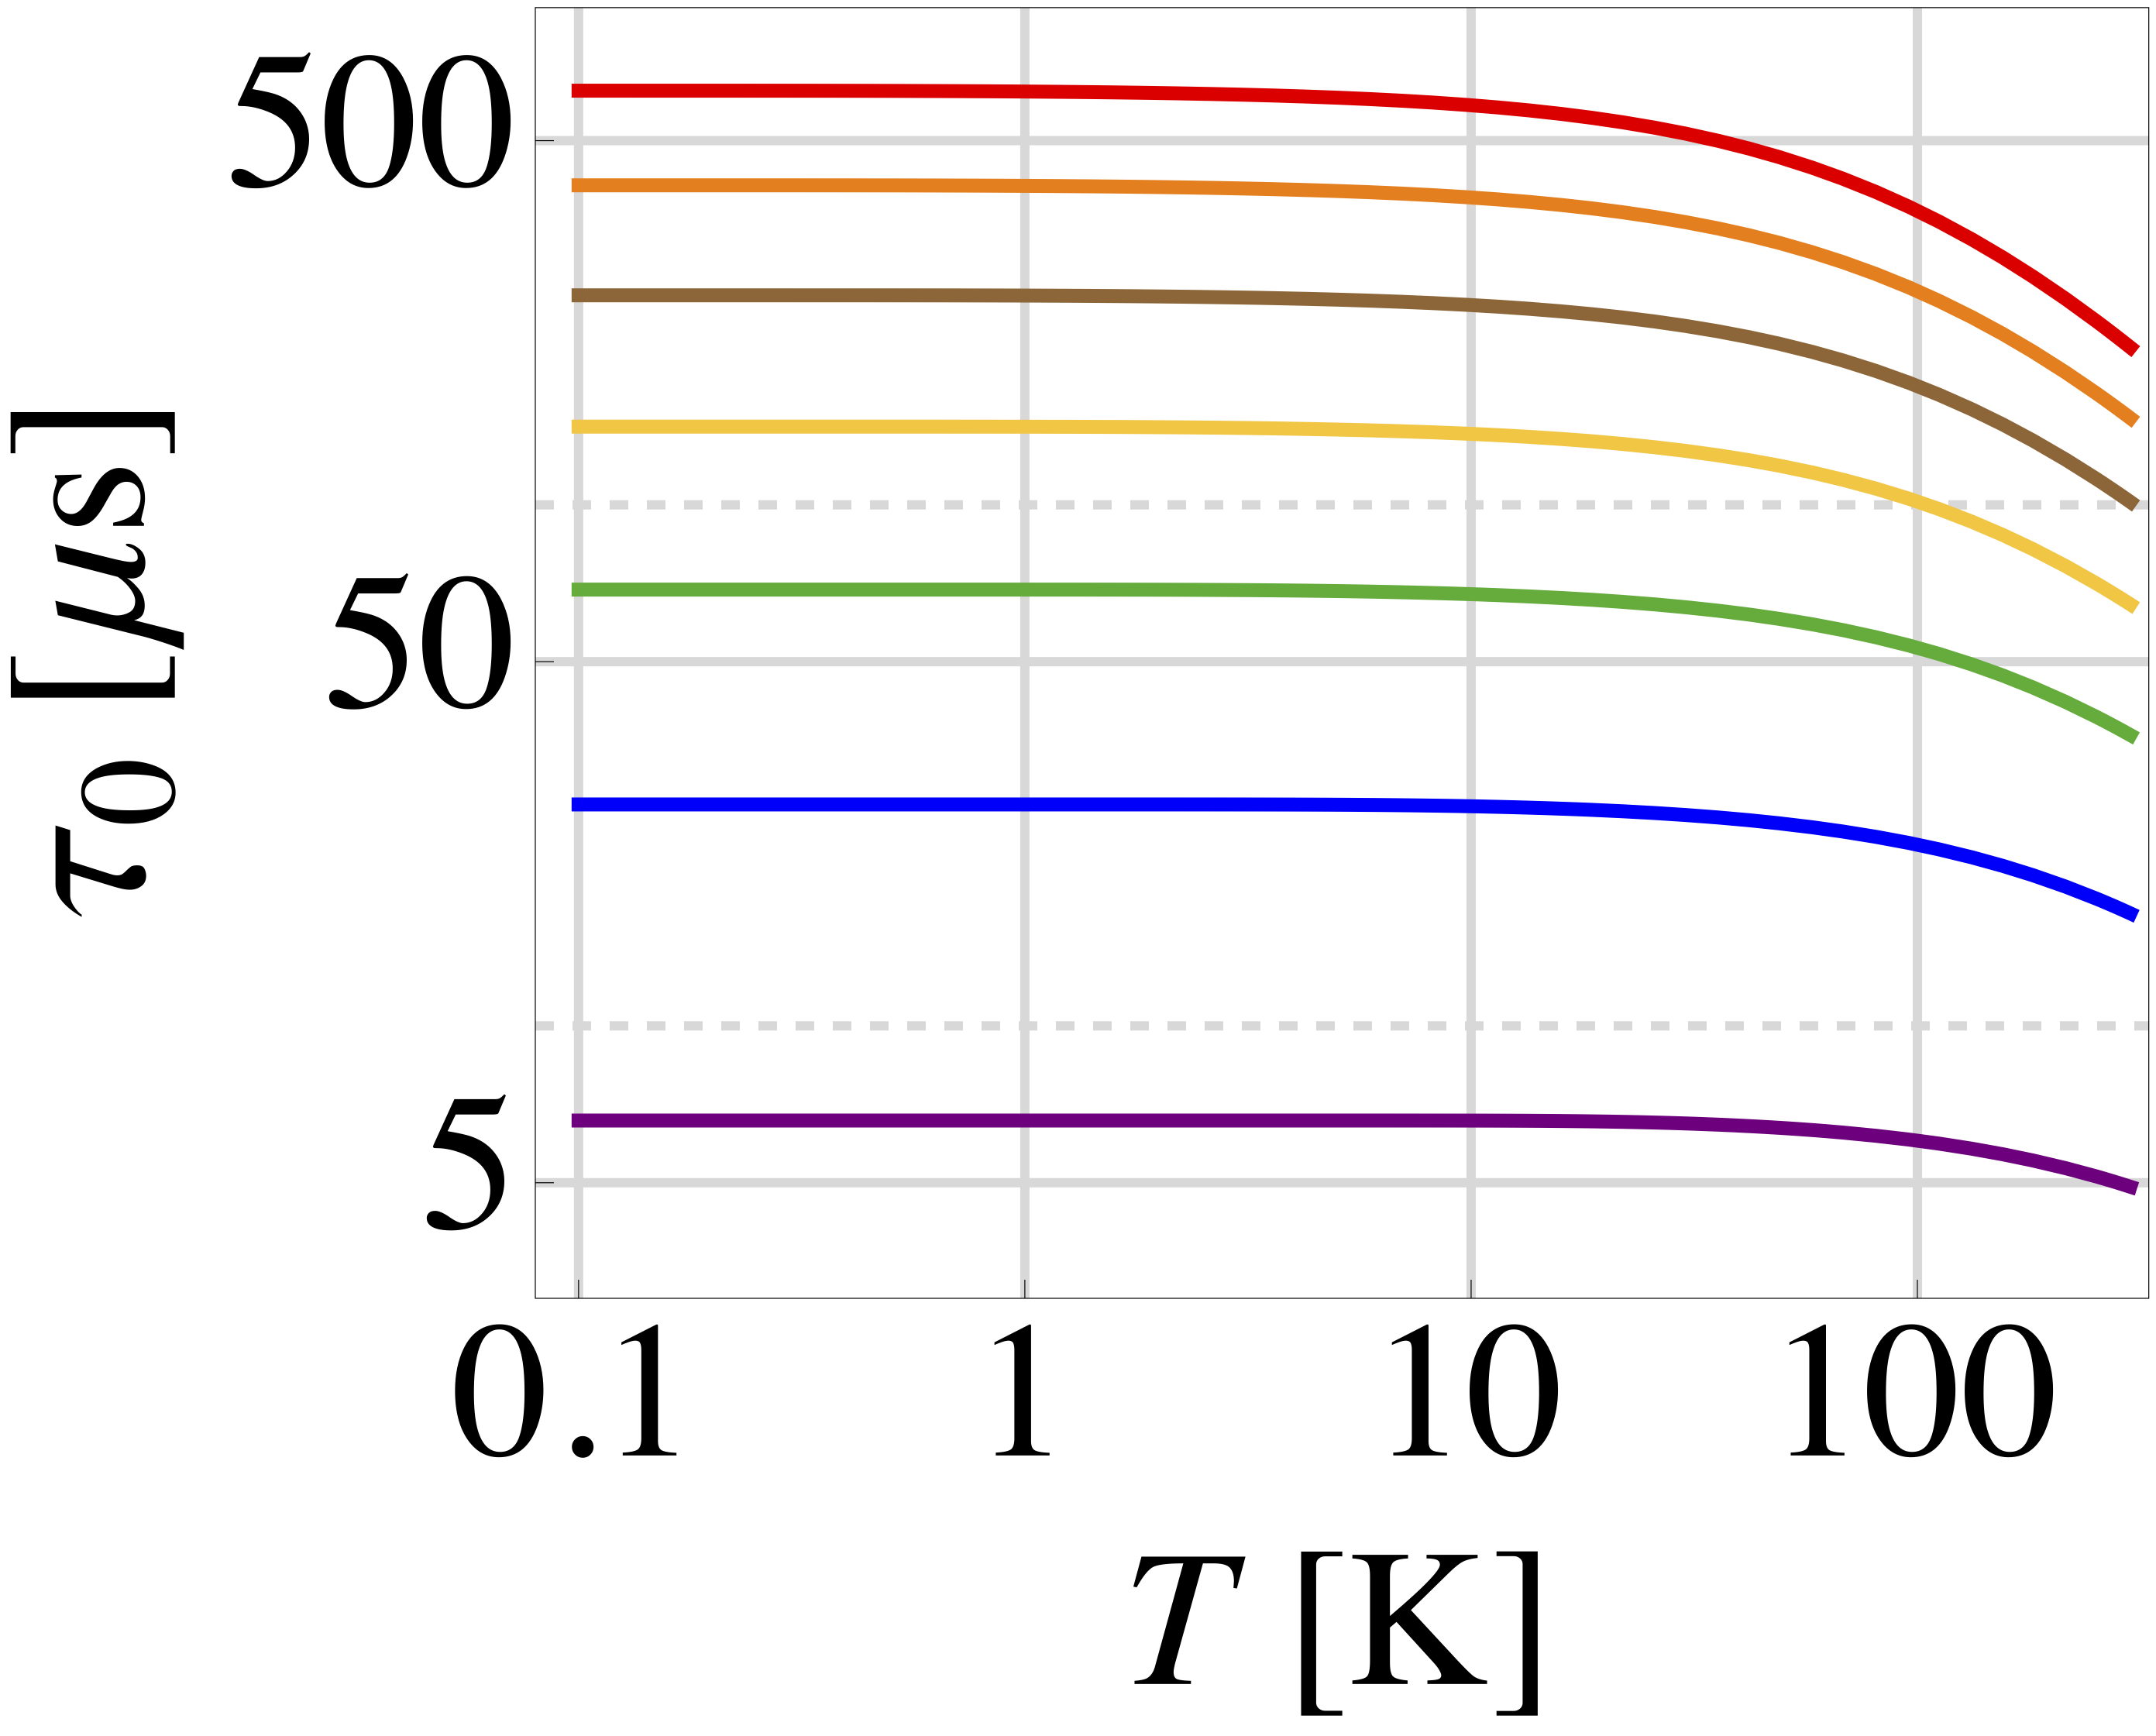
\includegraphics[width=2.5cm,height=2.3cm]{tauloglog.png}
  \subcaption{\iffalse$N^*_T$ vs $T$\fi}
  \label{fig:cthcal1_2}
  \vspace{0.3cm}
  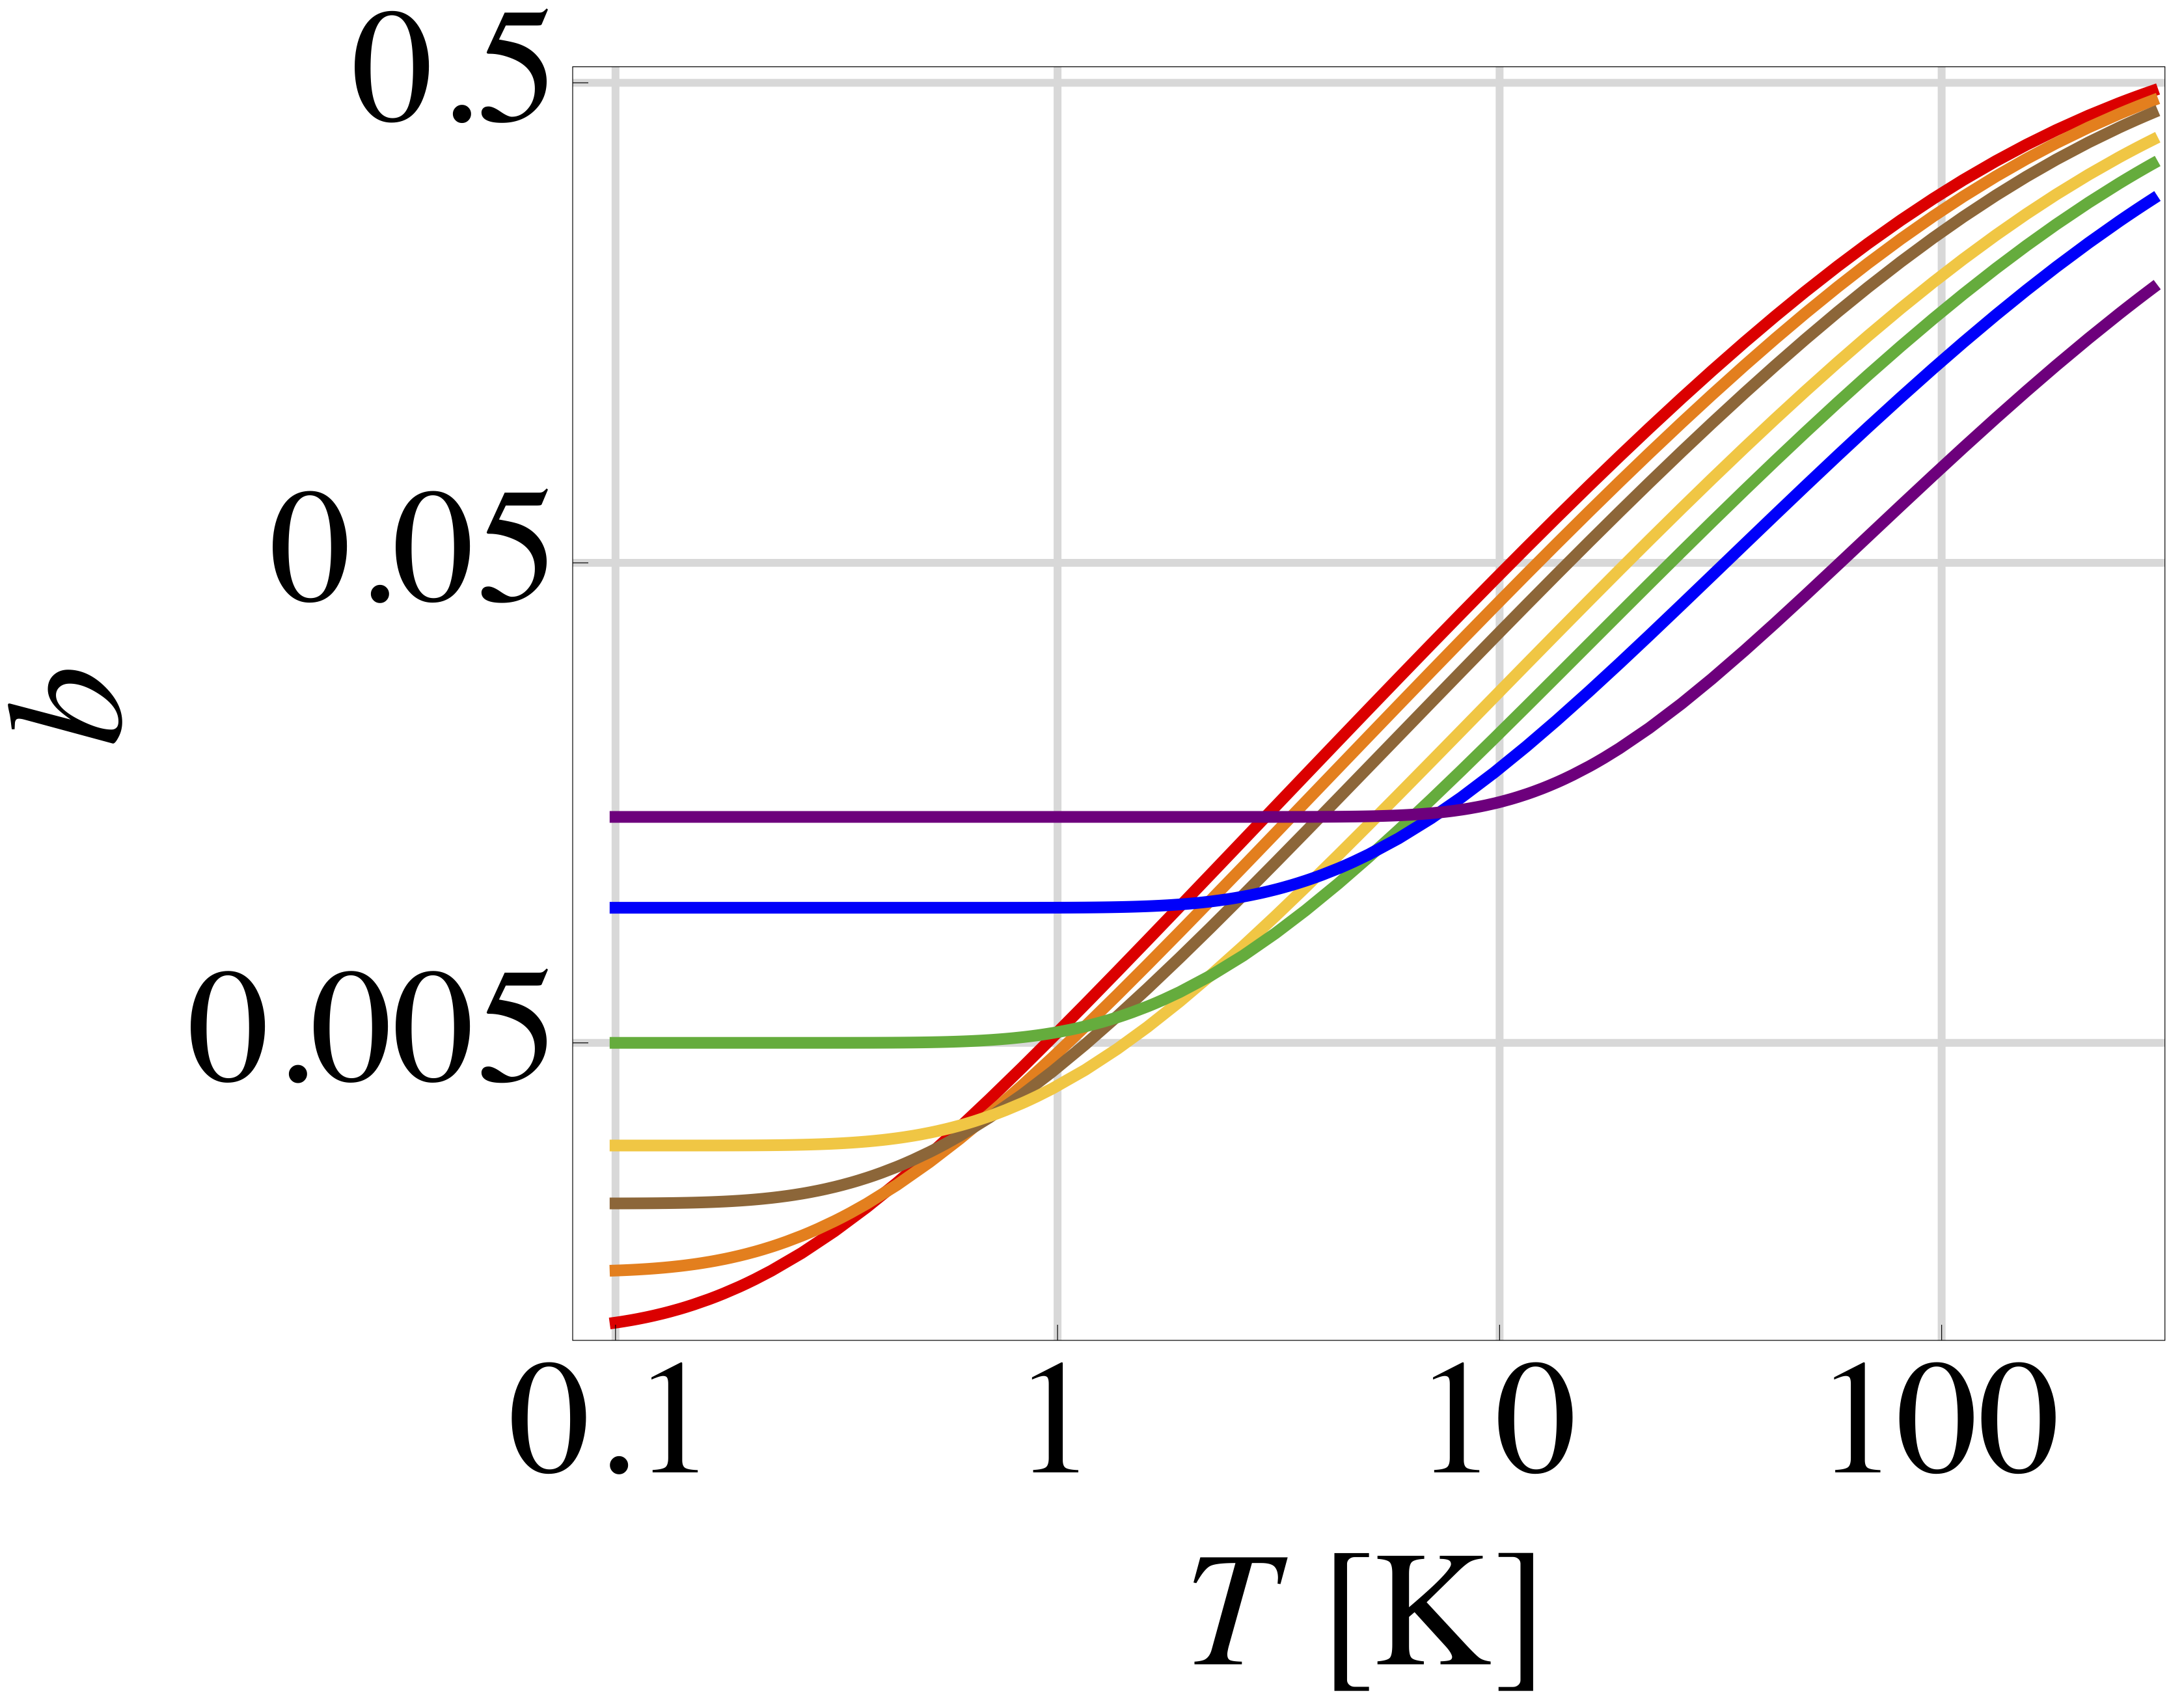
\includegraphics[width=2.5cm,height=2.3cm]{bloglog.png}
  \subcaption{\iffalse$N^*_T$ vs $T$\fi}
  \label{fig:cthcal2_2}
\end{minipage}
\begin{minipage}[r][6.4cm][t]{.33\textwidth}
  \vspace{\fill}
  \centering
  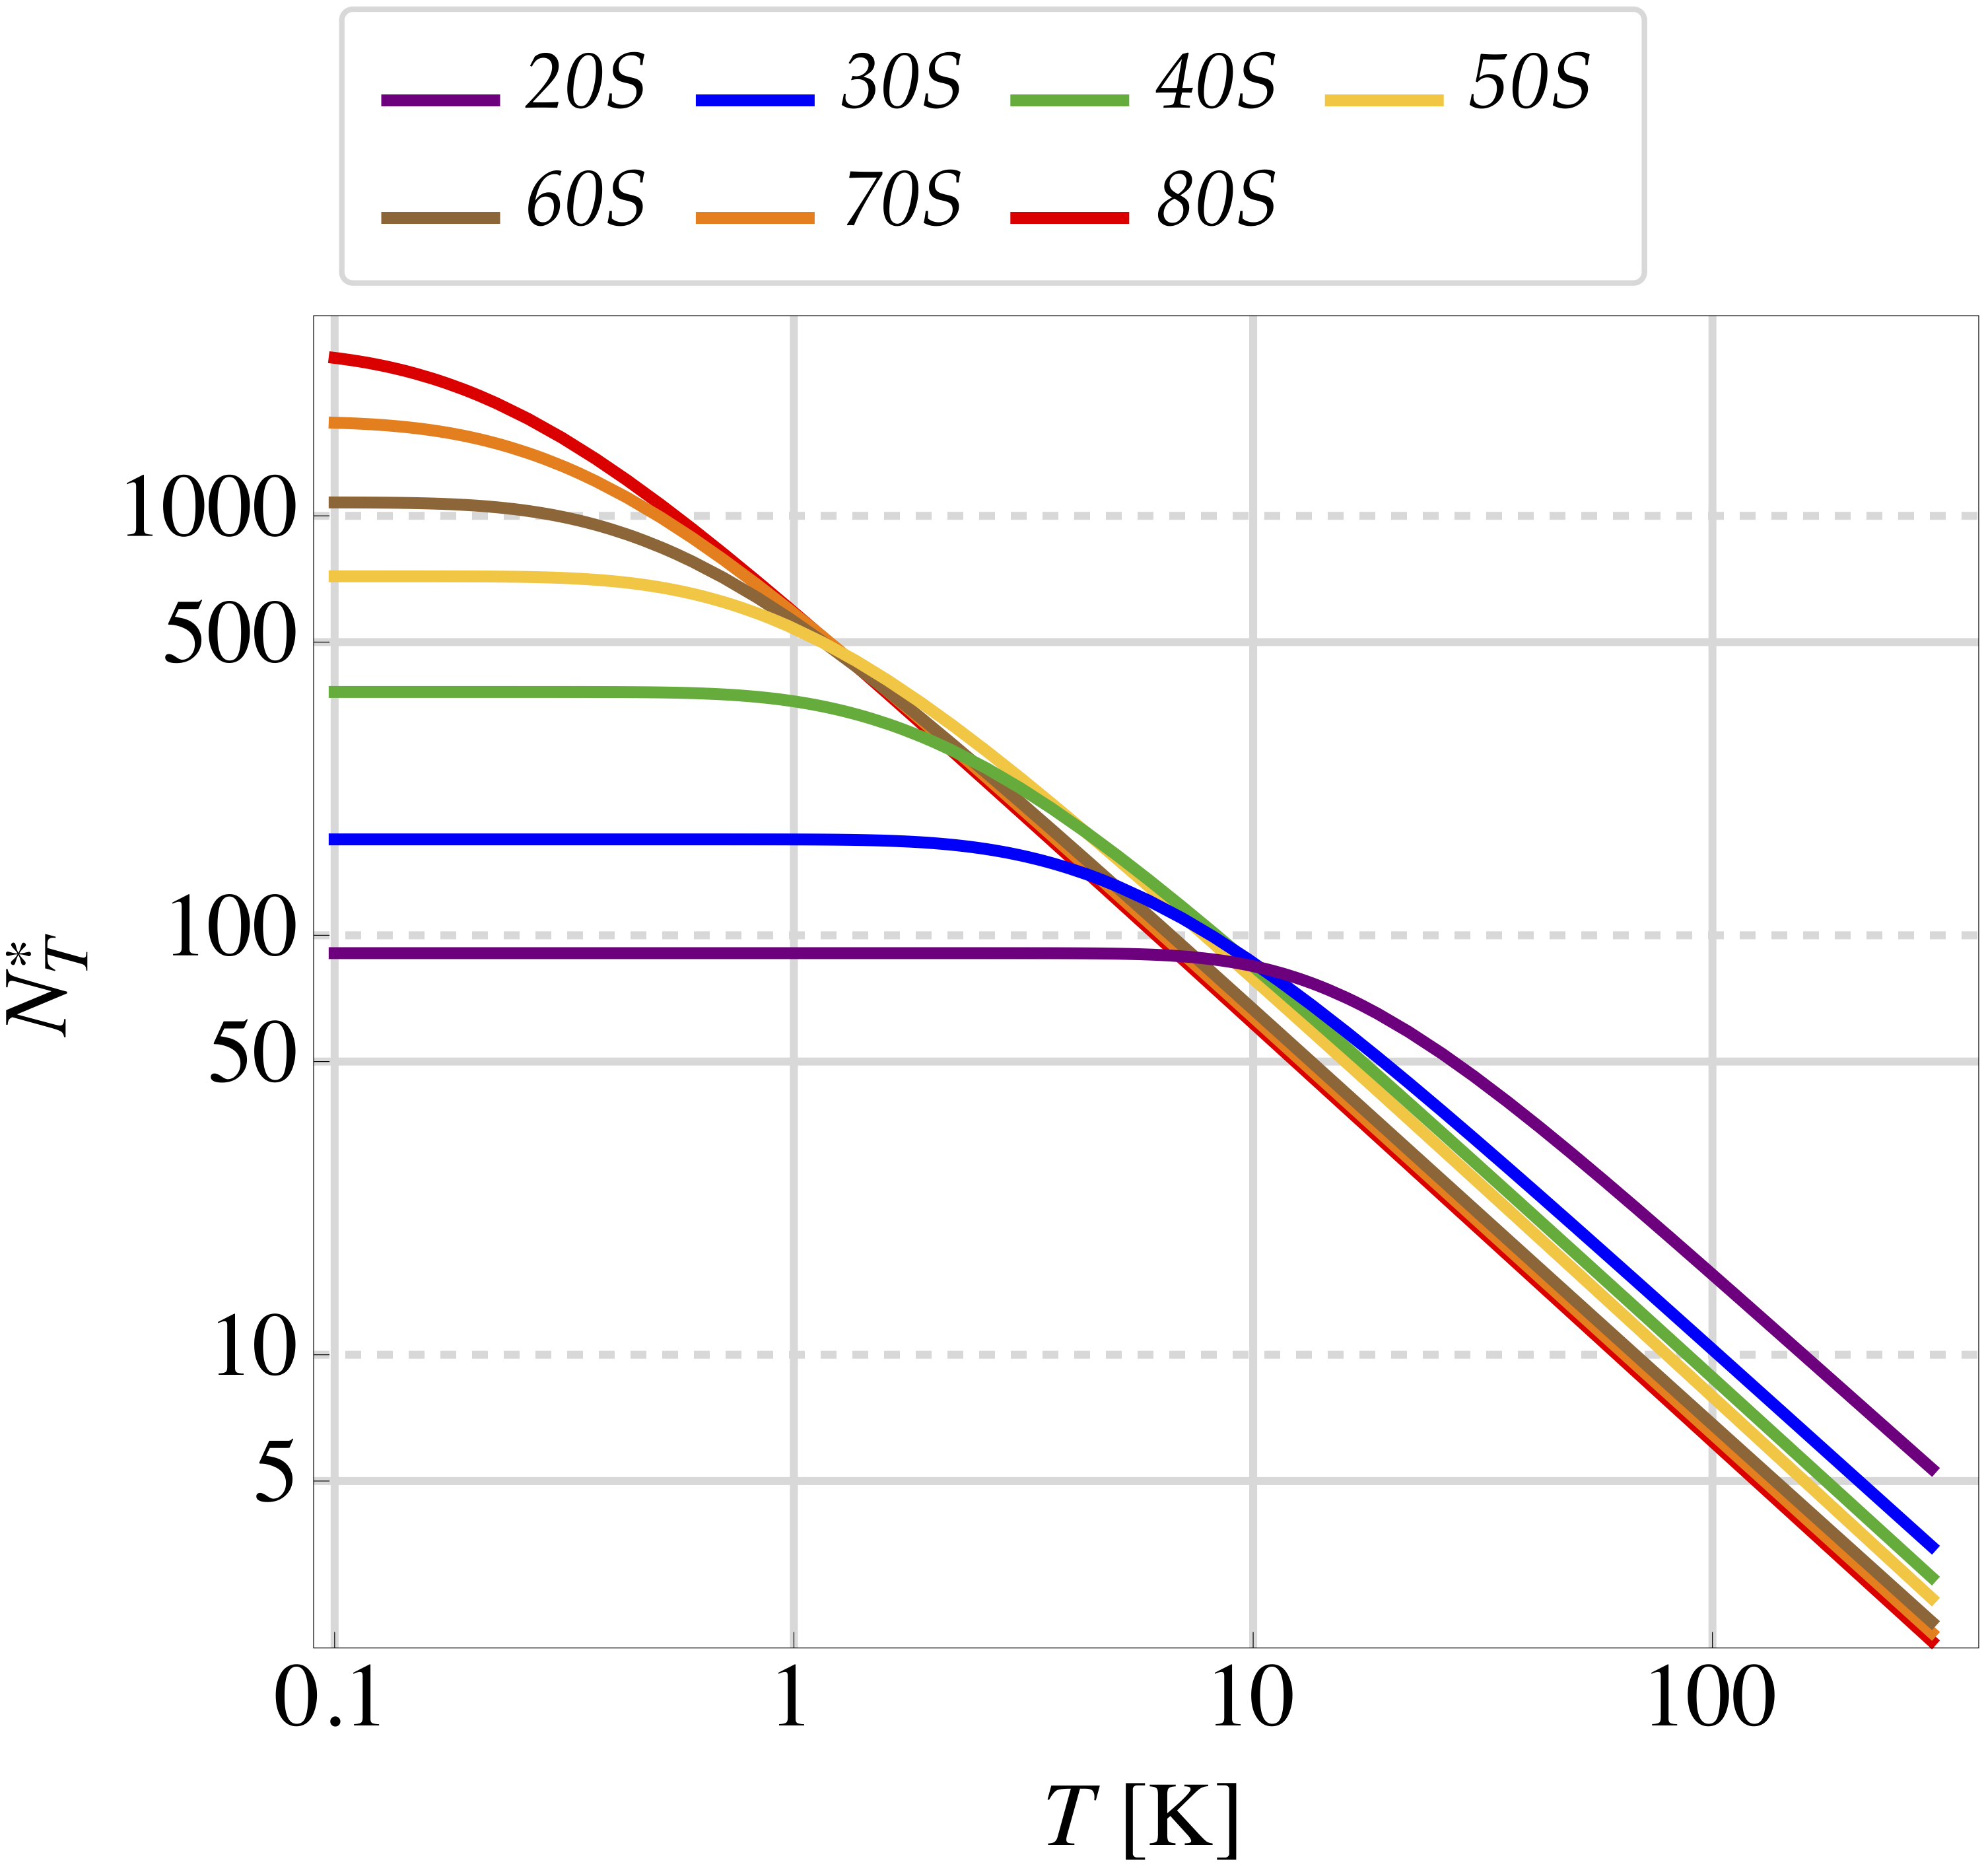
\includegraphics[width=5.9cm,height=5.7cm]{NTloglog2.png}
  \subcaption{\iffalse$N^*_T$ vs $T$\fi}
  \label{fig:cthcal3_2}
\end{minipage}%
\caption{(a). (b). (c) }
\end{figure}

\begin{figure}[]
\begin{minipage}[c][4.6cm][t]{.24\textwidth}
  \vspace*{\fill}
  \centering
  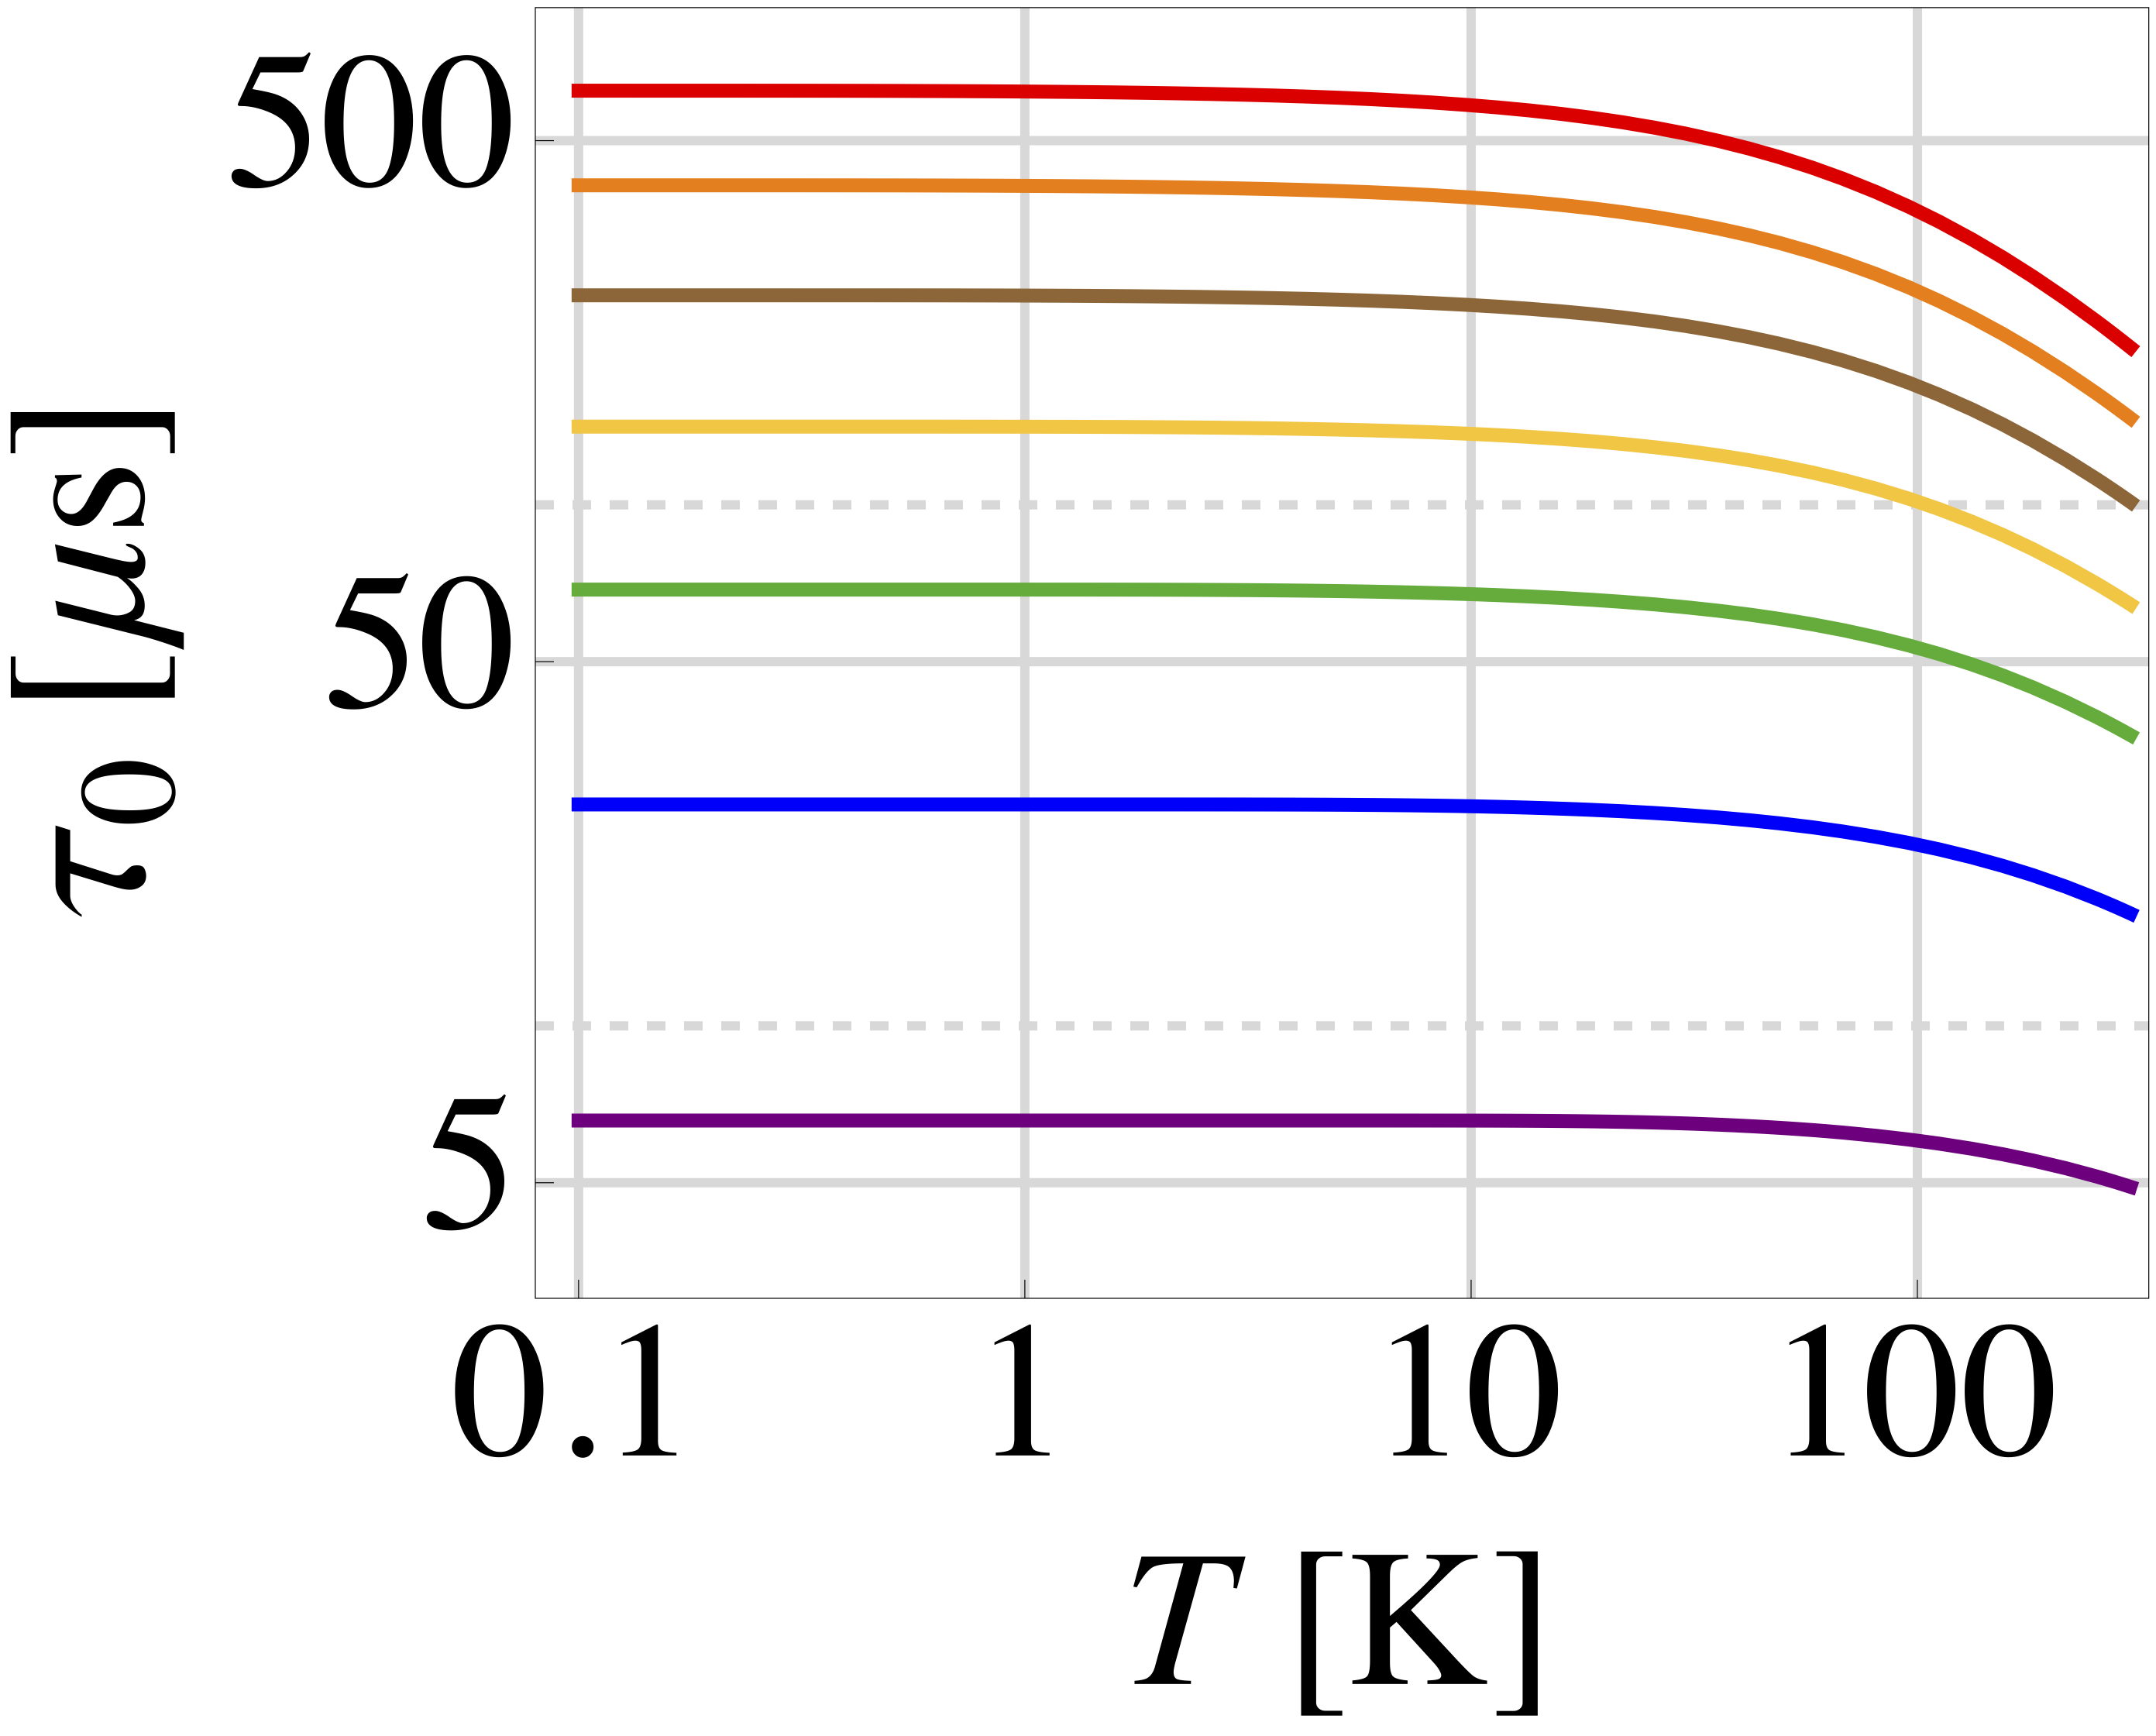
\includegraphics[width=3.8cm,height=3.2cm]{tauloglog.png}
  \subcaption{\iffalse$N^*_T$ vs $T$\fi}
  \label{fig:cthcal1_4}
  %
\end{minipage}%
\begin{minipage}[c][4.6cm][t]{.24\textwidth}
  \vspace*{\fill}
  \centering
  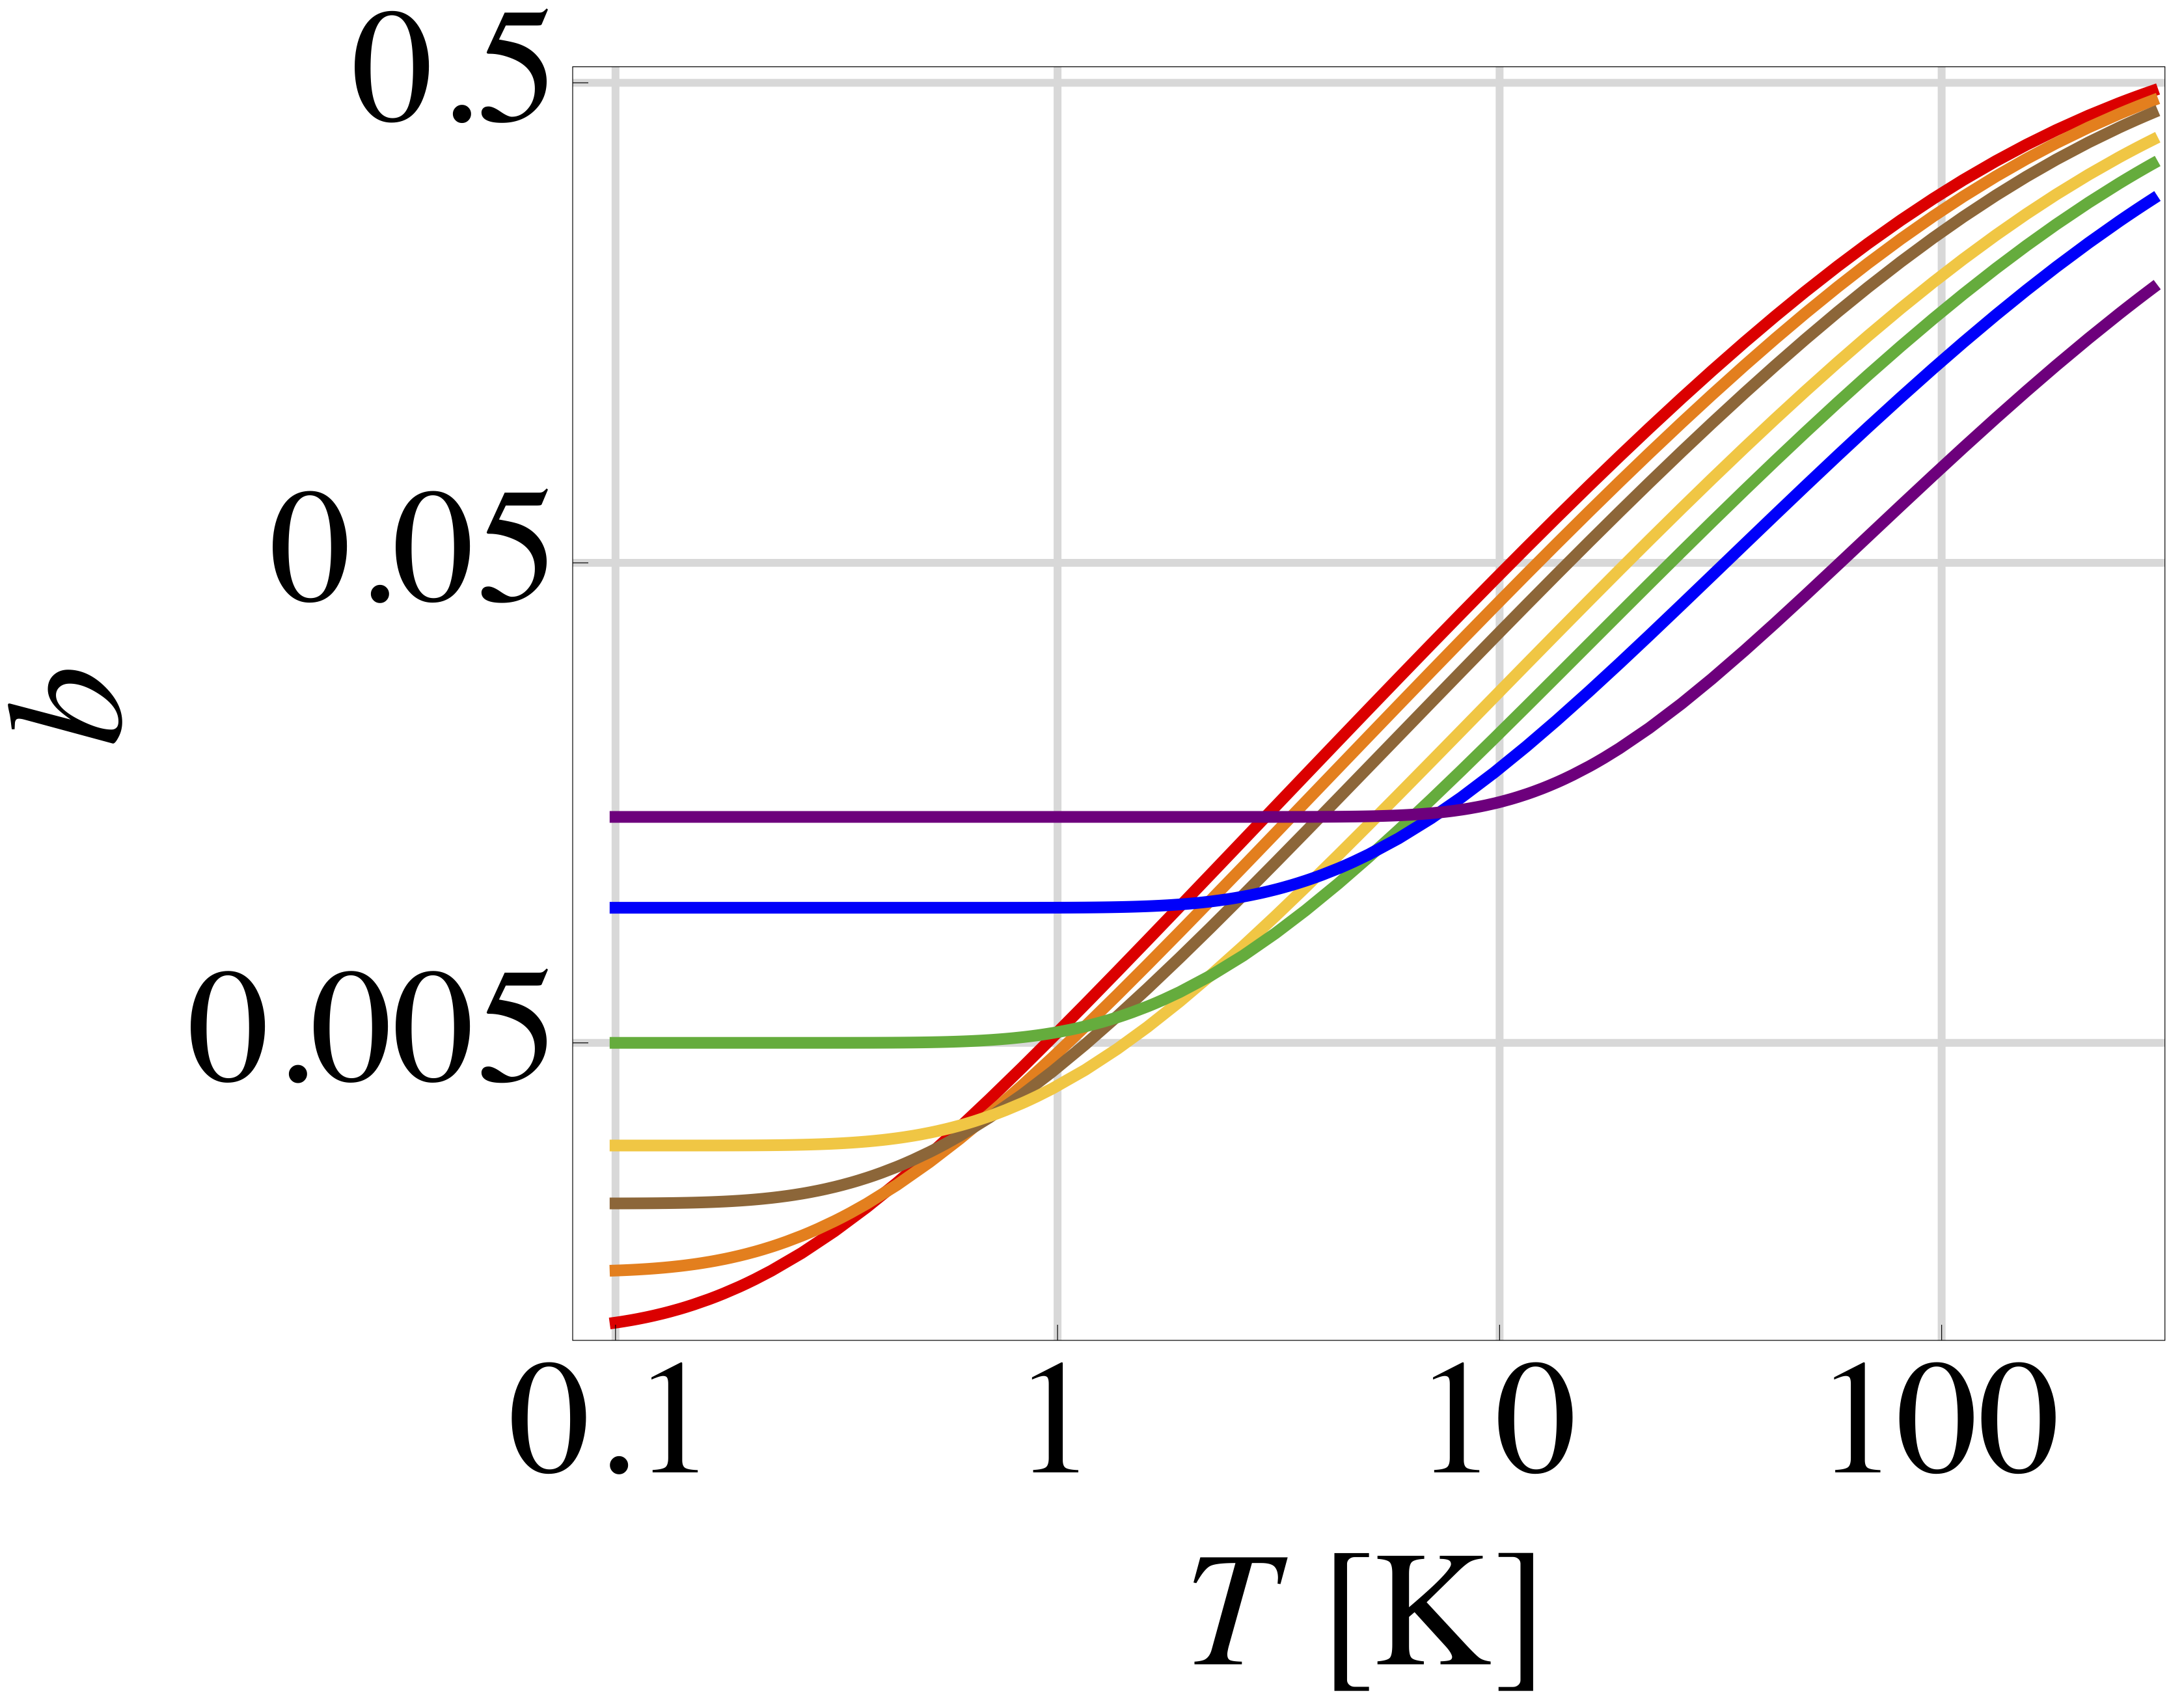
\includegraphics[width=3.8cm,height=3.2cm]{bloglog.png}
  \subcaption{\iffalse$N^*_T$ vs $T$\fi}
  \label{fig:cthcal2_4}
  %
\end{minipage}%
\vspace*{1.8cm}
\begin{minipage}[c][6cm][b]{.46\textwidth}
  \centering
  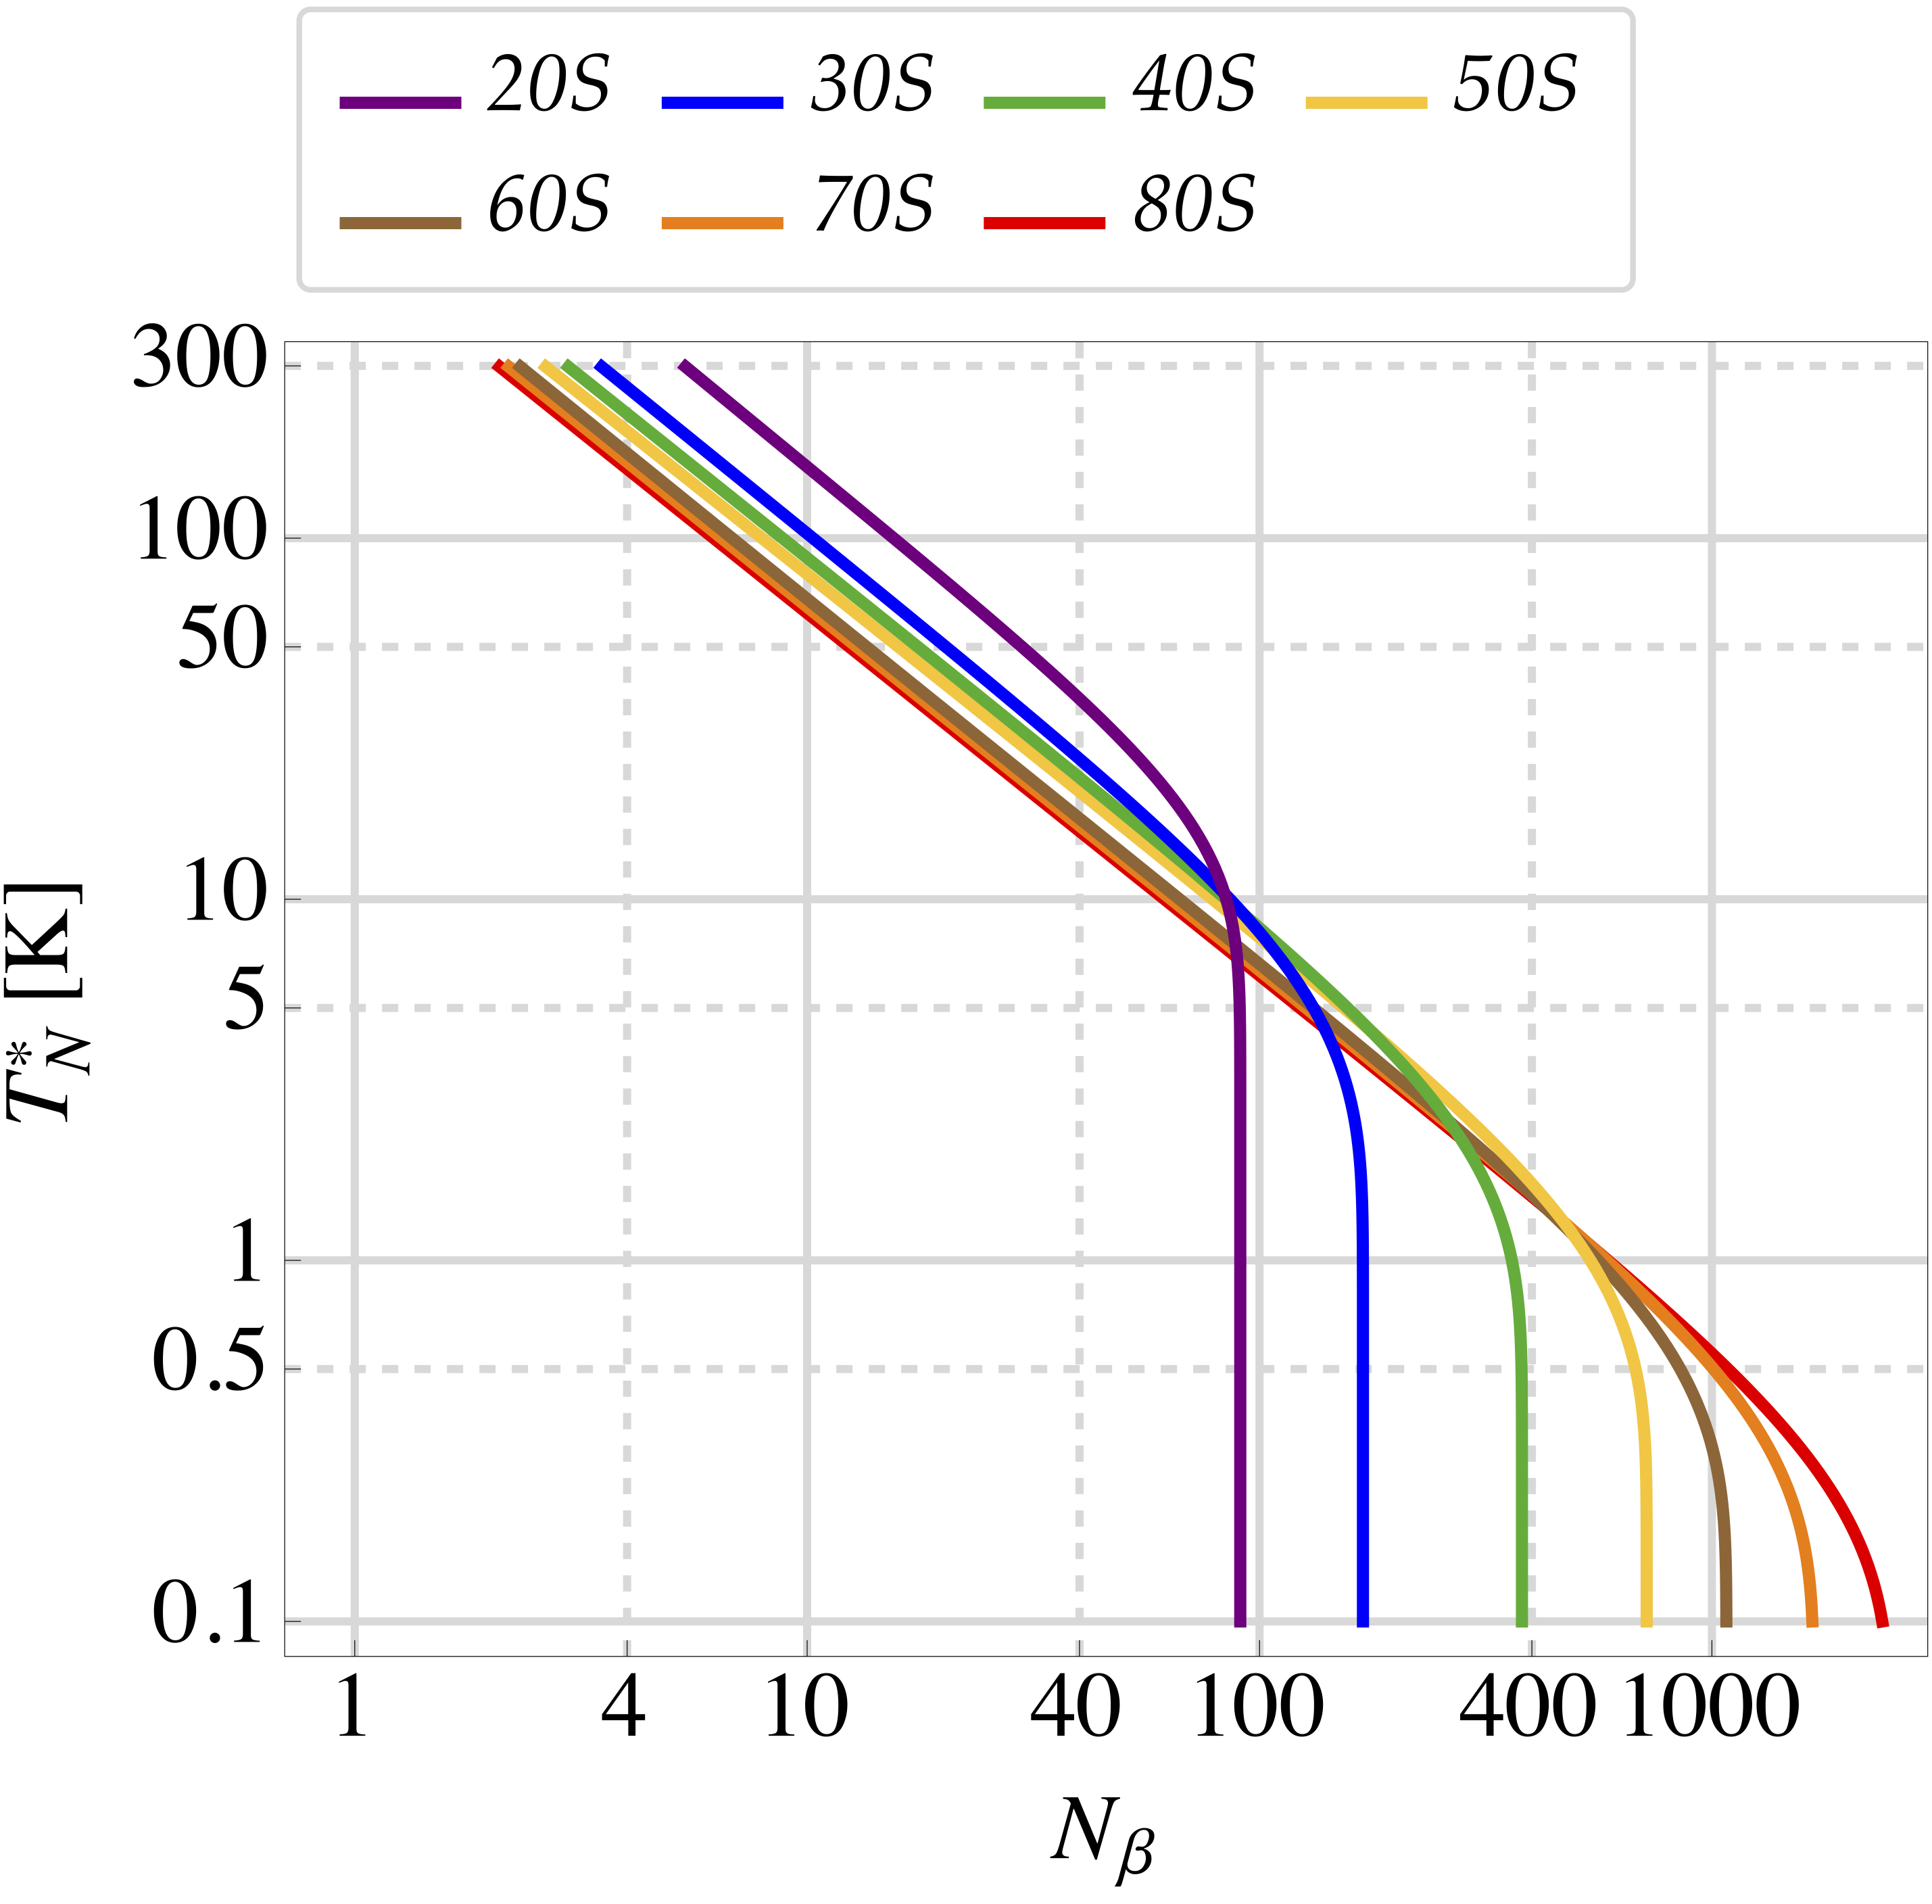
\includegraphics[width=7.0cm,height=6.8cm]{TvsNbloglog.png}
  \subcaption{\iffalse$N^*_T$ vs $T$\fi}
  \label{fig:cthcal3_4}
\end{minipage}
\caption{(a). (b). (c).}\label{fig:cthcal_4}
\end{figure}

\begin{thebibliography}{8}
\bibitem{ABp} 
AB paper.
 
\bibitem{Beterov} 
I. I. Beterov, I. I. Ryabtsev, D. B. Tretyakov, and V. M. Entin,
Phys. Rev. A 79, 052504 (2009).

\bibitem{Dyachkov}
L. G. Dyachkov and P. M. Pankratov, J. Phys. B 27, 461
(1994).

\bibitem{PupilloZollerSS} G. Pupillo, A. Micheli, M. Boninsegni, I. Lesanovsky, and
P. Zoller, Phys. Rev. Lett. 104, 223002 (2010).

\bibitem{Spin-Ice}  A. W. Glaetzle, M. Dalmonte, R. Nath, C. Gross, I. Bloch, and P. Zoller, Phys. Rev. Lett. 114, 173002 (2015).

\bibitem{BlochPaper} Zeiher-Bloch Paper. J. Zeiher, R. van Bijnen, P. Schauß, S. Hild, J.-y. Choi,
T. Pohl, I. Bloch, and C. Gross, Nature Physics (2016).

\bibitem{Soliton} PRL 106, 170401 (2011). Rydberg-Induced Solitons: Three-Dimensional Self-Trapping of Matter Waves

\bibitem{Heisenberg-limit} Physical Review Letters 116, 053601 (2016). Approaching the Heisenberg Limit without Single-Particle Detection.

\bibitem{van Bijnen} PRL 114, 243002 (2015). Quantum Magnetism and Topological Ordering via Rydberg Dressing near Forster Resonances.
 
\end{thebibliography}

\end{document}